\section{Study 5: remote emotion detection}
\label{s:experiment1-study5}

This study presents information regarding the use of machine learning to remotely detect the emotional state of subjects while they play a game. The literature review presented in chapters \ref{ch:literature-physiological}, \ref{ch:literature-face} and \ref{ch:literature-multifactorial} indicates that a model based on several user signals, which is a multifactorial analysis, is more efficient for emotion detection. The mentioned chapters also highlight which of those signals can be remotely acquired within the context of this research via computer vision techniques.

The majority of the previous work found in the literature mention the use of machine learning techniques to model user signals into emotional states \parencite{moghimi2017affective}. Different models and accuracy results are mentioned, which depend on several particularities of the approach used by the authors. Based on the literature, a neural network has been selected for this study as a promising machine learning model for affective recognition.

This study is a systematic evaluation of the feasibility of a user-tailored neural network trained on data samples from two calibration games of a given subject which is then used to classify samples from a third calibration game of that same subject. The following sections present how the study was conducted and analyzed, as well as the results obtained. Finally a discussion of the results and a conclusion is provided.

%%%%%%%%%%%%%%%%%%%%%%%%%%%%%%%%%%%%%%%%%%%%%%%%%%%%%%%%%%%%%%%%%%%%%%%%%
\subsection{Analysis and methods}
\label{s:experiment1-study5-method}
%%%%%%%%%%%%%%%%%%%%%%%%%%%%%%%%%%%%%%%%%%%%%%%%%%%%%%%%%%%%%%%%%%%%%%%%%

%%%%%%%%%%%%%%%%%%%%%%%%%%%%%%%%%%%%%%%%%%%%%%%%%%%%%%%%%%%%%%%%
\subsubsection{Data pre-processing}

The video recordings used in the present study are related to games designed to work as calibration games. Those calibration games feature a progression from a boring to a stressful state. That configuration is used as the foundation for the labeling process of emotional states during the training of the model, as well as ground truth for its testing.

\begin{figure}[ht]
    \centering
    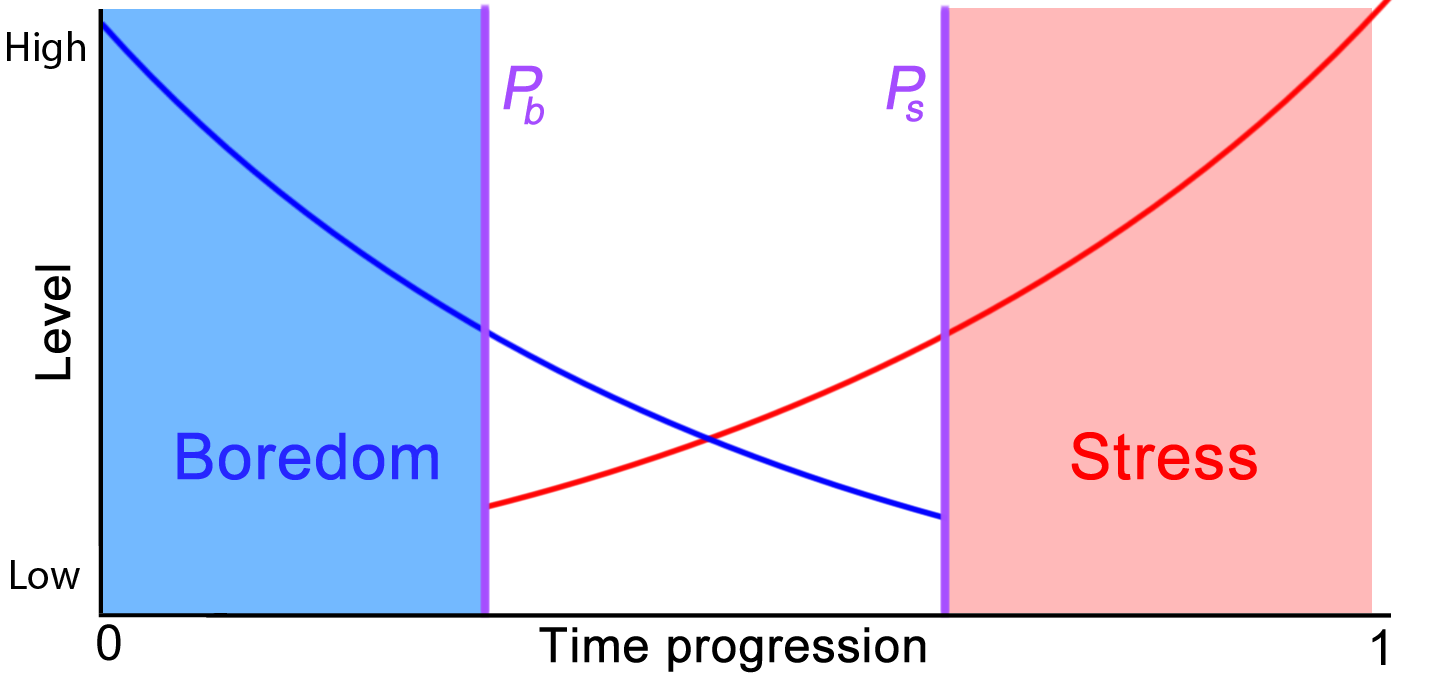
\includegraphics[width=0.95\textwidth]{figures/machine-learning-labeling-approach-B.png}
    \caption{Labeling approach for training/evauation of the user-tailored model based on varying points of division: $P_b$ (boredom samples) and $P_s$ (stress samples).}
    \label{fig:machine-learning-labeling-approach-B}
\end{figure}

Data used for training and evaluation of the emotion detection model is obtained according to the procedure illustrated in Figure \ref{fig:machine-learning-labeling-approach-B}. Each game is divided in two parts: boredom, i.e. $P_b$, and stress, i.e. $P_s$. Samples from the $P_s$ part are labeled as stress, while the samples from the $P_b$ part are labeled as boredom. The approach accounts for the informed levels of boredom and stress of the subject, labeling only the samples within the areas more likely to accurately reflect the self-reported emotional states.

In order to acomplish such division of data, a pre-processing step is applied. The pre-processing of video recordings involves the extraction of the parts containing the interaction with the games and the discard of noisy frames. The process is explained in details in Section \ref{s:experiment1-study4-feature-analysis} (on page \pageref{s:experiment1-study4-feature-analysis}). Firstly the periods where subjects were playing each one of the available games were extracted from the video recordings. It resulted in three videos per subject, denoted as $V_{s,i}$ where $s$ is the $s$-th subject and $i \in \{1, 2, 3\}$ represents the game. Then the initial 45 seconds of any given video $V_{s,i}$ were ignored. The remaining of the video was then divided into three pieces, from which the first and the last were selected as $H_0$ and $H_1$, respectively. Segment $H_0$ represents the boredom part, i.e. $P_b$, while $H_1$ represents the stressful part, i.e. $P_s$.

The pre-processing of the recordings resulted in 6 video segments per subjects: 3 segments $H_0$ (one per game) and 3 segments $H_1$ (one per game). A given game $i$ contains $N=20$ pairs of $H_0$ and $H_1$ video segments (20 segments $H_0$, one per subject, and 20 segments $H_1$, one per subject). When considering all subjects and games, there are $N=60$ pairs of $H_0$ and $H_1$ video segments (3 games $\times$ 20 subjects, resulting in 60 segments $H_0$ and 60 segments $H_1$). Subject 9 had problems playing the Platformer game, so all segments $H_0$ and $H_1$ from that subject were discarded. Consequentially there are $N=57$ pairs of $H_0$ and $H_1$ video segments in total after the pre-processing.

\subsubsection{Classification features}
%%%%%%%%%%%%%%%%%%%%%%%%%%%%%%%%%%%%%%%%%%%%%%%%%%%%%%%%%%%%%%%%%%%%%%%%%

The classification efficiency of a machine learning model is related to the number of features able to accurately discriminate the elements being classified. The use of more features does not necessarely produce a better model. Some features might not accurately contribute to the classification, which leads to degradation of results if they are included.

Features and their classification potential are highly dependent on the type of data being used. In the present study, the set of features used for classification was extracted and selected based on previous reports of the potential of said features to differentiate emotional states in games. In total 8 features, denoted $F_1$ to $F_8$, are available for use: $F_1$ to $F_7$ are related to facial activity, and $F_8$ and $F_9$ are related to HR activity, including remote estimations (rPPG). Table \ref{table:study5-features-list} presents a description of all features.

\begin{table*}
    \centering
    \caption{Description of features used for classification}
    \label{table:study5-features-list}
    \begin{tabular}[l]{@{}clp{6.5cm}}
        \hline
            \textbf{Notation} & \textbf{Name} & \textbf{Description} \\
        \hline
            $F_1$ & Mouth outer & Monitor the zygomatic muscle.  \\
            $F_2$ & Mouth corner & Monitor the zygomatic muscle. \\
            $F_3$ & Eye area & Monitor the orbicularis oculi muscle, e.g. blinking. \\
            $F_4$ & Eyebrow activity & Monitor the corrugator muscle.  \\
            $F_5$ & Face area & Monitor facial movement to and away from the camera  \\
            $F_6$ & Face motion & Describe the total distance the head has moved in any direction in a short period of time.  \\
            $F_7$ & Facial COM & Describe the overall movement of all facial landmarks. \\
            $F_8$ & Remote HR & HR estimated using the rPPG technique proposed by \textcite{poh2011advancements}.  \\
            $F_9$ & Ground HR & HR calculated from a physical sensor, i.e. watch. \\
        \hline
    \end{tabular}
\end{table*}

Features $F_1$ to $F_7$ are based on automatically detected facial landmarks related to facial elements that express a connection with emotional states. As previsouly mentioned in Chapter \ref{ch:literature-face}, there is evidence of more frequent corrugator activity when positive game events occur \parencite{hazlett2006measuring} and increased activity of zygomatic muscle associated with self-reported positive emotions \parencite{tijs2008dynamic}. Positive and rewarding game events are also connected to increase in zygomatic and orbicularis oculi activity \parencite{ravaja20051}. Detection of stress is also related to blinking rate \parencite{giannakakis2017stress,dinges2005optical}, lip movement \parencite{dinges2005optical} and lips deformation \parencite{metaxas2004image,giannakakis2017stress}, mouth activity \parencite{liao2005decision}, and head movement/velocity \parencite{giannakakis2017stress}.

Feature $F_8$ is based on remote estimations of HR performed using the rPPG technique proposed by \textcite{poh2011advancements}. Similarly feature $F_9$ is based on the HR readings provided by a physical sensor, i.e. watch, used by the subjects. As previously mentioned in Chapter \ref{ch:literature-physiological}, HR and its derivatives, such as HRV, have been used as reliable sources of information in different emotion estimation methods \parencite{kukolja2014comparative}. Reports in the literature show the use of HR and derivates for continuous arousal monitoring \parencite{grundlehner2009design}, measurement of confusion \parencite{xiao2015towards}, triangulation of phychophysiological emotional reactions to digital media stimuli \parencite{nogueira2015annotation}, detection of mental and physical stress \parencite{vandeput2009heart,garde2002effects}, and measurement of frustration \parencite{rodriguez2015vr}.

\subsubsection{Features extraction and calculation}
%%%%%%%%%%%%%%%%%%%%%%%%%%%%%%%%%%%%%%%%%%%%%%%%%%%%%%%%%%%%%%%%%%%%%%%%%

The process of extracting and calculating features is performed using a moving window applied on the videos of all subjects. The moving window has a size of 15 seconds and a step of 1 second (93.33\% overlap). For each window in the video, computer vision techniques are applied to all frames within that window to detect facial landmarks and to collect information regarding pixel values, e.g. mean value of pixels in the blue channel. The detected landmarks are used to calculate the features related to facial activity, while pixel values are used to estimate the HR.

Features $F_1$ to $F_7$, which represent facial activity, are mostly calculated using the Euclidian distance of automatically detected facial landmarks for each frame. A detailed description of the process is presented in Section \ref{s:study4} (page \pageref{s:study4}). Features $F_8$ and $F_9$, which represent HR activity, are calculated based on rPPG estimations of HR and on HR measurements of a physical sensor, respectively. A detailed description of the rPPG estimation process is presented in Section \ref{s:study3} (page \pageref{s:study3}).

Even though all frames within the window are analyzed, only a single, final value is assigned to each feature per window. For features $F_1$ to $F_7$, the final value of a given feature is calculated by aggregating the values of all frames within the window of that given feature using mean or standard deviation. From now on, $F_i^\mu$ and $F_i^\sigma$ will be used to denote feature $F_i$ whose values in a window were aggregated using mean and standard deviation, respectively. Empirical tests have shown that features connected to facial regions with fast changes within the window, e.g. eye area and face motion, are better represented with an aggregation using the standard deviation. Facial features with slower changes, e.g. face area and mouth activity, are better represented with an aggregation using the mean. Feature $F_8$ does not require any aggregation of values since all frames within the window are used to produce a single value, i.e. the estimation of the mean HR in that window. Finally feature $F_9$ is aggregated using the mean of all HR values provided by the physical sensor within the window, i.e. mean HR within the window.

\subsubsection{Training and evaluation of an emotion classifier}
\label{s:experiment1-study5-training-evaluation}
%%%%%%%%%%%%%%%%%%%%%%%%%%%%%%%%%%%%%%%%%%%%%%%%%%%%%%%%%%%%%%%%%%%%%%%%%

The classification procedure uses the previously mentioned feature set and a neural network trained to identify two emotional states: boredom and stress. Both the training and evaluation of the neural network are performed on a user tailored fashion: data from a given subject $S_i$ is used to train and evaluate the emotion classification of that given subject $S_i$. Figure \ref{fig:study5-training-evaluation} illustrates the process.

\begin{figure}[ht]
    \centering
    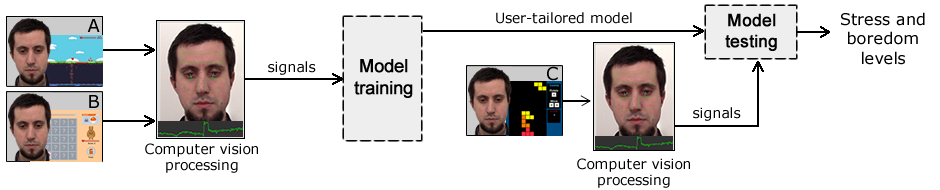
\includegraphics[width=\textwidth]{figures/machine-learning-investigation.png}
    \caption{Iteration of a 3-fold \textit{Leave One Session Out Cross Validation} performed on a gaming sessions with 3 games, i.e. A, B and C. Data of two calibration games, e.g. A and B, are used to train the machine learning model, while data of the third calibration game, e.g. C, is used to evaluate the model.}
    \label{fig:study5-training-evaluation}
\end{figure}

Leave One Session Out Cross Validation (LOSOCV) is used to evaluate each trained user-tailored model, as illustrated in Figure \ref{fig:study5-training-evaluation}. In LOSOCV, data from one session instance is left out and a model is constructed on data from all other session instances. In the present study, a given subject $S_i$ played 3 calibration games, e.g. A, B and C, so data from one calibration game is left out and a model is trained on the data of the other two calibration games for that subject $S_i$. This is repeated for all three calibration games of that subject $S_i$. Consequentially the use of LOSOCV will produce 3 models per subject, resulting in 3 measurements of classificaiton accuracy per subject, denoted $L_j$, where $j \in \{1, 2, 3\}$ represent each evaluated model. The final classification accuracy for given subject $S_i$, named $A_i$, is calculated as the mean of $L_j$ values obtained from the iterations in the LOSOCV. In other words, each subject contributes a single classification accuracy value $A_i$, which is calculated based on the mean classification accuracy of his/her three models in the LOSOCV iterations.

In the training process of each model, which is performed 3 times per user, the hyper-parameters of each neural network, e.g. number of neurons, is optimized using random search \parencite{bergstra2012random}. A 10-fold cross validation method repeated 3 times is applied, so the dataset is split into 10-subsets and each of those subset is held out while the model is trained on all others. The process is repeated 3 times and the final metric for the model is the mean from the number of repeats. Area under the ROC curve (AUC) is used as a metric to select the best model.

According to previous analysis, subjects perceived the games as being boring at the beginning and stressful at the end. As a consequence, it is assumed that subject's emotional state in $H_0$ and $H_1$ is boredom and stress, respectively. Based on that assumption, training and evaluation data obtained from video segments in $H_0$ and $H_1$ were labeld as boredom and stress, respectively.

%, which finds models as good or beter then ones configured by a pure grid search

%Describe how the model was trained, which includes how the calibration games were grouped, e.g. two for training, one for testing. Explain that neural networks were used because they are widely mentioned in the literature.

%%%%%%%%%%%%%%%%%%%%%%%%%%%%%%%%%%%%%%%%%%%%%%%%%%%%%%%%%%%%%%%%%%%%%%%%
\subsubsection{Analysis}
\label{s:experiment1-study5-analysis}
%%%%%%%%%%%%%%%%%%%%%%%%%%%%%%%%%%%%%%%%%%%%%%%%%%%%%%%%%%%%%%%%%%%%%%%%%

In order to test the effectiveness of the neural network in classifying samples as either boredom or stress, all trained neural networks were evaluated in conjunction. As described in the previous section, each subject's model was evaluated using LOSOCV, which produced a classification accuracy $A_i$ for any given subject $S_i$. The minimum, maximum and mean value of $A_i$ was calculated as a metric for accuracy. In order to provide better contextualization of the classification results, the same process was also applied to other three metrics obtained during the LOSOCV evaluation: precision, recall and F1 score.

Aiming to better understand the contribution of each feature for the classification process, the training/evaluation process mentioned early was also performed using different feature sets. Each of those different feature sets was evaluated in an independent test, denoted $T_i$. Table \ref{table:study5-different-feature-sets} shows tests $T_i$ and the corresponding feature sets used in the process.

\begin{table*}
    \centering
    \caption{Tests and their respective feature sets}
    \label{table:study5-different-feature-sets}
    \begin{tabular}[l]{@{}cclp{4.0cm}}
        \hline
            \textbf{$T_i$} & \textbf{Name} & \textbf{Feature set} & \textbf{Note} \\
        \hline
            1 & \texttt{MULTI\_R} & $F_1^\mu$, $F_2^\mu$, $F_3^\sigma$, $F_4^\sigma$, $F_5^\mu$, $F_6^\sigma$, $F_8$ & Facial analysis, rPPG-estimated HR.\\ % 5278d175-71e752ce: HR_poh2011, mean_face_activity_mouth_corner, mean_face_activity_mouth_outer, mean_face_area, std_face_activity_eyebrow, std_face_eye_area, std_face_motion_instability
            2 & \texttt{MULTI\_G} & $F_1^\mu$, $F_2^\mu$, $F_3^\sigma$, $F_4^\sigma$, $F_5^\mu$, $F_6^\sigma$, $F_9^\mu$ & Facial analysis, HR from physical sensor.\\ % 5278d175-9fa716ee: mean_HR_ground, mean_face_activity_mouth_corner, mean_face_activity_mouth_outer, mean_face_area, std_face_activity_eyebrow, std_face_eye_area, std_face_motion_instability
            3 & \texttt{FACE} & $F_1^\mu$, $F_2^\mu$, $F_3^\sigma$, $F_4^\sigma$, $F_5^\mu$, $F_6^\sigma$ & Facial analysis only. \\ % 5278d175-826512b2: mean_face_activity_mouth_corner, mean_face_activity_mouth_outer, mean_face_area, std_face_activity_eyebrow, std_face_eye_area, std_face_motion_instability
            4 & \texttt{HR\_R} & $F_8$ & rPPG-estimated HR only.\\ % 5278d175-97a38001: HR_poh2011
            5 & \texttt{HR\_G} & $F_9^\mu$ & HR from physical sensor only. \\ % 5278d175-ad2580a5: mean_HR_ground
        \hline
    \end{tabular}
\end{table*}

Tests \texttt{MULTI\_R} and \texttt{MULTI\_G} use multifactorial set of features for their neural network, where facial and HR information are used in combination. The difference between \texttt{MULTI\_R} and \texttt{MULTI\_G} is that the former uses rPPG estimated HR, while the latter uses HR obtained from the physical sensor. Test \texttt{FACE} uses a set of features based solely on facial information. Finally tests \texttt{HR\_R} and \texttt{HR\_G} use only HR information as a feature. Similarly to \texttt{MULTI\_R} and \texttt{MULTI\_G}, tests \texttt{HR\_R} and \texttt{HR\_G} use HR readings from rPPG estimatations and from a physical sensor, respectively.

Subjects perceived the games as boring and stressful, so such difference should make a trained neural network capable of properly classifying evaluation samples as either boredom or stress. Additionally the use of a multifactorial approach, where facial analysis and HR information are used in combination instead of either one alone, is expected to produce better classification results \parencite{zacharatos2014automatic}. Based on those expectations, the following hypotheses are stated:

\begin{itemize}
  \item $u_1$: a user-tailored neural network trained on data samples from two calibration games of a given subject $S_i$ is able to classify samples from a third calibration game of that same subject $S_i$ with an accuracy greater than chance-level rate (random guessing);
  \item $u_2$: a user-tailored neural network using a multifactorial feature set, i.e. facial and HR features, performs with greater accuracy than a user-tailored neural network using facial features only;
  \item $u_3$: a user-tailored neural network using a multifactorial feature set, i.e. facial and HR features, performs with greater accuracy than a user-tailored neural network using HR features only.
\end{itemize}

Hypothesis $u_1$ was tested by checking if the mean value of the classification accuracy, i.e. calculated from all $A_i$ values, is greater than 0.5. In such case it is assumed that an accuracy rate of 0.5 (50\%) is the theoretical probabilistic chance level achieved by totally random classification performed by a classifier evaluated on an infinite number of data samples. Hypotheses $u_2$ and $u_3$ were tested by performing a Wilcoxon Signed Ranks test on all $J_i$ values of the two competing tests $T_i$. As previously mentioned, the use of LOSOCV produces 57 accuracy measuraments $J_i$ per test $T_i$.

%%%%%%%%%%%%%%%%%%%%%%%%%%%%%%%%%%%%%%%%%%%%%%%%%%%%%%%%%%%%%%%%%%%%%%%%%
\subsection{Results}
%%%%%%%%%%%%%%%%%%%%%%%%%%%%%%%%%%%%%%%%%%%%%%%%%%%%%%%%%%%%%%%%%%%%%%%%%

Table \ref{table:study5-result-metrics-mean} presents the mean values of the resulting classification metrics for accuracy, precision, recall and F1 score, calculated and analyzed according to the procedures described in Section \ref{s:experiment1-study5-method}. Regarding the accuracy metric, the highest mean value achieved was 62.3\% in test \texttt{MULTI\_G}, whose model used a combination of facial and HR features. The HR feature in that case was calculated from the physical sensor, not remotely estimated. The second and third highest accuracy rates were 60.8\% in test \texttt{HR\_G} (HR from physical sensor only) and 60.4\% in test \texttt{MULTI\_R} (facial and remotely-estimared HR features), respectively. The highest values achieved for precision, recall and F1 score were 65.6\%, 62.4\%, and 58.1\%, respectively, all in test \texttt{HR\_G}.

\begin{table*}
    \centering
    \caption{Mean values of resulting classification metrics}
    \label{table:study5-result-metrics-mean}
    \begin{tabular}[l]{@{}ccccc}
        \hline
            \textbf{Test} & \textbf{Accuracy} & \textbf{Precision} & \textbf{Recall} & \textbf{F1}\\
        \hline
            \texttt{MULTI\_R} & 0.604 & 0.612 & 0.599 & 0.521 \\ % 5278d175-71e752ce
            \texttt{MULTI\_G} & \textbf{0.623} & 0.583 & 0.607 & 0.514 \\ % 5278d175-9fa716ee
            \texttt{FACE} & 0.594 & 0.601 & 0.585 & 0.507 \\ % 5278d175-826512b2
            \texttt{HR\_R} & 0.547 & 0.541 & 0.545 & 0.497 \\ % 5278d175-97a38001
            \texttt{HR\_G} & 0.608 & \textbf{0.656} & \textbf{0.624} & \textbf{0.581} \\ % 5278d175-ad2580a5
        \hline
    \end{tabular}
\end{table*}

Table \ref{table:study5-result-metrics-minmax} presents a discrimination of the minumum and maximum mean values for the resulting classification metrics. At least one subject in test \texttt{MULTI\_G} has been classified with a mean accuracy of 98\%, the highest value for that metric in all tests. The worst mean accuracy value was 19\% for at least one subject in test \texttt{MULTI\_R}. Regarding precision, the highest mean value was 97\% in test \texttt{MULTI\_G}. In all tests but \texttt{HR\_G}, at least one subject has been classified with zero precision (all samples were classified wrongly). Regarding precision, the highest and lowest mean values were 98\% and 12\% in tests \texttt{MULTI\_G} and \texttt{FACE}, respectively. Finally regarding F1 score, the highest mean value was 98\% for at least one subject in test \texttt{MULTI\_G}. All tests presented zero as the lowest F1 score.

\begin{table}[!htbp]
  \centering
  \caption{Minimum and maximum mean values of resulting classification metrics}
  \label{table:study5-result-metrics-minmax}
  \begin{tabular}{ccccccccc}
    \hline
      \textbf{Test} & \multicolumn{2}{c}{\textbf{Accuracy}} & \multicolumn{2}{c}{\textbf{Precision}} & \multicolumn{2}{c}{\textbf{Recall}} & \multicolumn{2}{c}{\textbf{F1}} \\
      {} & min & max & min & max & min & max & min & max \\
    \hline
      \texttt{MULTI\_R}  & 0.19 & 0.91 & 0.00 & 0.95 & 0.19 & 0.87 & 0.00 & 0.91 \\ % 5278d175-71e752ce
      \texttt{MULTI\_G}  & 0.25 & \textbf{0.98} & 0.00 & \textbf{0.97} & 0.13 & \textbf{0.98} & 0.00 & \textbf{0.98} \\ % 5278d175-9fa716ee
      \texttt{FACE}  & 0.26 & 0.90 & 0.00 & 0.95 & 0.12 & 0.90 & 0.00 & 0.89 \\ % 5278d175-826512b2
      \texttt{HR\_R}  & 0.36 & 0.72 & 0.00 & 0.79 & 0.18 & 0.77 & 0.00 & 0.67 \\ % 5278d175-97a38001
      \texttt{HR\_G}  & 0.38 & 0.82 & 0.26 & 0.85 & 0.23 & 0.87 & 0.00 & 0.81 \\ % 5278d175-ad2580a5
    \hline
  \end{tabular}
\end{table}

% data_multi_r and data_hr_r: p = 0.04488, Zstat = -2.0058, effect = 0.2657
% data_multi_r and data_face: p = 0.26797, Zstat = -1.1077, effect = 0.1467

Finally there are indications that a multifactorial model, which uses a combination of facial and HR features, performs with greater accuracy than a model using either facial or HR features. A Wilcoxon Signed Ranks test indicates that the mean accuracy was greater for a multifactorial model using facial and remotely estimated HR features, i.e. \texttt{MULTI\_R}, than for a model using only remotely estimated HR, i.e. \texttt{HR\_R}, $Z=-2.00$, $p=0.044$, $r=0.26$. However there are no indications that the mean accuracy of such multifactorial model, i.e. \texttt{MULTI\_R}, is statistically significantly greater than the mean accuracy of a model using only facil features, i.e. \texttt{FACE}, $Z=-1.10$, $p=0.267$, $r=0.14$.

%%%%%%%%%%%%%%%%%%%%%%%%%%%%%%%%%%%%%%%%%%%%%%%%%%%%%%%%%%%%%%%%%%%%%%%%%
\subsection{Discussion}
%%%%%%%%%%%%%%%%%%%%%%%%%%%%%%%%%%%%%%%%%%%%%%%%%%%%%%%%%%%%%%%%%%%%%%%%%

% data_multi_g and data_face: p = 0.03343, Zstat = -2.1269, effect = 0.2817
% data_multi_g and data_hr_g: p = 0.27802, Zstat = -1.0848, effect = 0.1437

% data_multi_g and data_multi_r: p = 0.07836, Zstat = -1.7603, effect = 0.2332

Results indicate that the use of a user-tailored model to remotely estimate the emotional state of players from videos of gaming sessions is feasible. Previously mentioned hypothesis $u_1$ states that a user-tailored neural network trained on data samples from two calibration games of a given subject $S_i$ is able to classify samples from a third calibration game of that same subject $S_i$ with an accuracy greater than chance-level rate (random guessing). Such model was tested in two configurations: \texttt{MULTI\_R} and \texttt{MULTI\_G}. Model \texttt{MULTI\_R}, which uses a multifactorial feature set composed of facial and remotely estimated HR information, presented a mean classification accuracy of 60.4\%. Such reported accuracy is greater than 50\%, the theoretical probabilistic chance level, which confirms hypothesis $u_1$. Model \texttt{MULTI\_G}, which also uses a multifactorial feature set but differs in the acquisition of HR data, i.e. physical sensor instead of remote estimation, presented a mean classification accuracy of 62.3\%. Such reported accuracy is also greater than the theoretical probabilistic chance level. The slightly greater classification accuracy of model \texttt{MULTI\_G} compared to \texttt{MULTI\_R} suggests that more precise rPPG estimations of the HR could improve the overall classification accuracy of model \texttt{MULTI\_R}. A Wilcoxon Signed Ranks test, however, has no statistically significant indication that the accuracy was greater for \texttt{MULTI\_G} than for \texttt{MULTI\_R}, $Z=-1.76$, $p=0.078$, $r=0.23$. Despite not being statistically signiciant, values $p=0.078$ and $r=0.23$ (small effect according to Cohen's classification of effect size) suggest a trend towards that reasoning.

Hypothesis $u_2$ states that a user-tailored neural network using a multifactorial feature set performs with greater accuracy than a user-tailored neural network using facial features only. The Wilcoxon Signed Ranks test mentioned in the previous section presented no statistically significant indications that the classification accuracy of \texttt{MULTI\_R} is greater than \texttt{FACE}. Such results refute hypothesis $u_2$ and suggest that a set of facial features, e.g. eyebrow and mouth analysis, has a greater potential to differentiate emotional states in a classifier. Particuarly it could perform better than a classifier based on rPPG-estimated HR alone, in the context of this experiment.

Regarding hypothesis $u_3$, which states that a user-tailored neural network using a multifactorial feature set performs with greater accuracy than a user-tailored neural network using HR features only. The Wilcoxon Signed Ranks test mentioned in the previous section presents statistically significant indications that the classification accuracy of \texttt{MULTI\_R} is greater than \texttt{HR\_R}. It supports the claim of hypothesis $u_3$, confirming that a multifactorial model performs better than one based solely on remotely estimated HR data. The lower classification potential of remotely estimated HR, however, could be attributed to errors in the rPPG estimation process caused by noise, e.g. natural movement of subjects (see Section \ref{s:study3}, on page \pageref{s:study3}, for more information). As a consequence, a more precise HR estimation used in a multifactorial model allegedly contributes to produce a better classifier. A Wilcoxon Signed Ranks test confirms with statistical significance that the classification accuracy of \texttt{MULTI\_G}, i.e. facial and HR from sensor, is greater than the accuracy of \texttt{FACE}, i.e. facial information only, $Z=-2.12$, $p=0.033$, $r=0.28$. It supports the previously mentioned idea that a precise HR estimation (from a physical sensor in the case of \texttt{MULTI\_G}) combined with facial information is a better classifier than one using facial information alone, i.e. model \texttt{FACE}. Finally a Wilcoxon Signed Ranks test does not indicate that the accuracy of \texttt{MULTI\_G} is greater than \texttt{HR\_G}, $Z=-1.08$, $p=0.278$, $r=0.14$. Consequentially it seems that precise estimations of HR is important, but HR or facial information used separatedely are likely to be less important for classification then a joint, multifactorial use of them in the emotion classification process.

Finally it is important to highlight the possible limitations of using the theoretical probabilistic chance level rate of 50\% for the evaluation of the model's accuracy. As previously mentioned, an accuracy baseline of 50\% assumes a totally random classification evaluated on an infinite number of data samples. One could argue that such scenario is unrealistic. In that case, the true evaluation of a model must consider statistical significance levels taking into account the sample size used in the process. \textcite{combrisson2015exceeding} present a work in the field of brain signal classification that uses analytical and empirical solutions, i.e. binomial formula and permutation tests, to show the influence of small numbers of data samples in the theoretical probabilistic chance level. According to the authors, a minimal correct classification rate of 62.5\% is required to assert statistial significance, i.e. $p < 0.05$, during the classification of two classes with a sample size of 40. In the present study, each subject was evaluated with 38 samples on average\footnote{This number refers to the amount of samples used for the evaluation of a model, not its training. During the training phase of each model, more than 38 samples were used per subject.}. As presented in the results of this study, the mean accuracy rate of models \texttt{MULTI\_R} and \texttt{MULTI\_G} are 60.4\% and 62.3\%, respectively. Following the analysis of \textcite{combrisson2015exceeding}, the mean accuracy rate of those multifactorial models would not be enough to assert statistical significance of the results. Nevertheless both models presented a mean accuracy that is considerably close to the minimal 62.5\%. Additionally the previously mentioned Wilcoxon Signed Ranks test does not indicate that the accuracy was greater for \texttt{MULTI\_G} than for \texttt{MULTI\_R}, so their performance could be the same. It is also important to stress the use of Leave One Session Out Cross Validation in the evaluation of each subject. It uses a completely independent and different game as source of sampling for the evaluation of each model, which strengthens the evaluation process. The reduced number of subjects in the study, i.e. 19, and the reduced number of samples used in the evaluation of each models, i.e. 38 on average, are in fact limiting factors. Reported results, however, provide insights regarding the feasibility of a multifactorial remote approach for emotion classification. The accuracy of the models presented in this study are not statistically confirmed without the assumption of baseline produced by a random classifier evaluated on an infinite number of data samples. However there is in fact a trend indicating that the use of a user-tailored model to remotely estimate emotional states of players is worth of further investigation.

% From: https://www.sciencedirect.com/science/article/pii/S1053811916000604#bb0235
% Recently, Combrisson and Jerbi (2015) compared the various statistical tests used to evaluate decoding performance and showed that the theoretical chance level was less stringent for small numbers of data samples, as found in neuroimaging studies, causing a bias towards statistical significance. The permutation test, by contrast, is not open to this criticism because it is a data-driven method and does not make assumptions about the statistical properties of the dataset. Therefore, the significance test we used may have been more stringent than the one used by those obtaining positive decoding findings in FFA.

%%%%%%%%%%%%%%%%%%%%%%%%%%%%%%%%%%%%%%%%%%%%%%%%%%%%%%%%%%%%%%%%%%%%%%%%%
\subsection{Conclusions}
%%%%%%%%%%%%%%%%%%%%%%%%%%%%%%%%%%%%%%%%%%%%%%%%%%%%%%%%%%%%%%%%%%%%%%%%%

This study presented a systematic evaluation of the feasibility of using a user-tailored neural network trained on data samples from two calibration games of a given subject to classify emotional states from a third calibration game of that same subject. Results support the idea that a user-tailored neural network, based on remotely acquired data from video recordings, is able to classify emotional states with an accuracy greater than chance-level rate (random guessing).

Regarding the efficienty of a multifactorial model, where facial and HR information are together instead of separatedely, there are no statistically significant indications that the classification accuracy of such a model is greater than a model using facial information alone. However a multifactorial model based on remotely acquired data performs better than one based solely on remotely estimated HR data.

Finally it seems that precise estimations of HR is important, but HR or facial information used separatedely are likely to be less important for classification then a combined use of them in a multifactorial emotion classification model based on remotely acquired data. The analysis performed in this study supports further investigation regarding a user-tailored model to remotely estimate emotional states of player.
